% \documentclass{article}

\documentclass{article}
%% \documentclass[twocolumn]{article}

\renewcommand{\familydefault}{\sfdefault} % Standardfont ändern auf Sans Serif (bny)

\usepackage[utf8x]{inputenc}
\usepackage[german]{babel} % Sprache umschalten /hat funktioniert bis auf Authors, bny 13.04.2016
\usepackage{tcolorbox}
\usepackage{xcolor}
\definecolor{chamois}{rgb}{1,.984314,.956863}  % RGB 255 247 231
\pagecolor{chamois}
\usepackage{geometry}
\geometry{verbose,a4paper,tmargin=10mm,bmargin=10mm,lmargin=10mm,rmargin=10mm}

\usepackage{multicol} % 20.04.2017 hinzugefügt, bny

%%% \usepackage{tikz}
%%% % \pagecolor{olive!50!yellow!50!white}

%% --> Hinweis, 11.08.2017, bny
%% --> Multicol ist nur zuständig für Spalten, die farbigen Kacheln werden mit tcolorbox gemacht
%% --> soll nur eine einspaltige Box eingefügt werden, wird multicol auskommandiert. (siehe Beschaffung)

\tcbuselibrary{skins}

\colorlet{xlightblue}{blue!5}

\newtcolorbox{beamerlikethm}[1]{
  title=#1,
  beamer,
  % colback=xlightblue,
  colframe=red!50,
  fonttitle=\bfseries,
  left=1mm,
  right=1mm,
  top=1mm,
  bottom=1mm,
  middle=1mm
}


\begin{document}
\pagestyle{empty}

%%% \begin{tikzpicture}[remember picture, overlay]
%%% \shade[left color=red!50,
%%% right color=green!50
%%% ] (current page.north west) rectangle (current page.south east);
%%% \end{tikzpicture}

\centering{{\huge Classement des documents}}

\vspace{\baselineskip}

%%%%%%

% \begin{beamerlikethm}{Eine Sitzungseinladung bearbeiten}
% \begin{itemize}
%   \item[$\Longrightarrow$] Wählen Sie die gewünschte Sitzung aus. Klicken Sie auf den Titel. Die Optionen öffnen sich.
%  \item[$\Longrightarrow$] Klicken Sie auf das Bearbeitungssymbol. Nun können Sie die gewünschten Änderungen vornehmen.
%   \item[$\Longrightarrow$] Schliessend Sie den Vorgang erneut mit Klick auf 'Übernahme' ab.
% \end{itemize}
% \end{beamerlikethm}


%%%% Box 1+2 in zwei Spalten

\begin{multicols}{2}

\begin{tcolorbox}[colback=blue!5,colframe=blue!40!black,title=Charger des documents]
\begin{itemize}
  \item[$\Longrightarrow$] Cliquez sur le symbole 
\includegraphics[height=10pt]{Icons/Plussymbol.jpg}, et un masque de saisie s'affiche.
  \item[$\Longrightarrow$] Ajoutez le fichier désiré dans le champ 'Fichier' ou saisissez un lien dans le champ 'Adresse'.
  \item[$\Longrightarrow$] Complétez les autres champs de saisie.
  \item[$\Longrightarrow$] Pour pouvoir sauvegarder le document, vous devez d'abord définir au moins un droit d'accès. 
	\item[$\Longrightarrow$] Cliquez sur le symbole 
\includegraphics[height=10pt]{Icons/Pluszeichen.jpg} et ajoutez un groupe ou un utilisateur avec les accès désirés.
	\item[$\Longrightarrow$] Pour terminer, cliquez sur le bouton 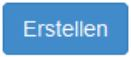
\includegraphics[height=12pt]{Icons/B_Erstellen.jpg}.
\end{itemize}
\end{tcolorbox}


\begin{tcolorbox}[colback=blue!5,colframe=blue!40!black,title=Associer des documents à Google-Maps]
\begin{itemize}
  \item[$\Longrightarrow$] Choisissez un document et cliquez sur le symbole de modification 
\includegraphics[height=10pt]{Icons/bearbeiten.jpg}.
  \item[$\Longrightarrow$] En haut à gauche, cliquez sur 'Afficher / masquer carte'. La carte Google-Maps est affichée.
  \item[$\Longrightarrow$] Cliquez et glissez la carte pour déplacer la section de carte. Utilisez la roue de votre souris pour faire un zoom en avant ou en arrière.
  \item[$\Longrightarrow$] Faites un double-clic à l'endroit désiré. Une épingle 
\includegraphics[height=10pt]{Icons/vNadel.jpg} signale l'endroit auquel le document est associé.
	\item[$\Longrightarrow$] Vous pouvez toujours déplacer l'épingle 
\includegraphics[height=10pt]{Icons/vNadel.jpg} ou la supprimer par un clic droit.
\end{itemize}
\end{tcolorbox}


\end{multicols}

%%%% Box 3+4 in zwei Spalten

\begin{multicols}{2}

\begin{tcolorbox}[colback=blue!5,colframe=blue!40!black,title=Extraire des documents pour les modifier en ligne]
\begin{itemize}
  \item[$\Longrightarrow$] Choisissez un document de la liste des documents et cliquez sur son titre. Des options s'affichent.
  \item[$\Longrightarrow$] Cliquez sur le symbole 
\includegraphics[height=12pt]{Icons/Auschecken.jpg}. Le document est extrait et ouvert.
  \item[$\Longrightarrow$] Modifiez le document et cliquez sur 
\includegraphics[height=12pt]{Icons/Sync2013.jpg} ou 
\includegraphics[height=12pt]{Icons/Sync2016.jpg} pour sauvegarder vos modifications. Le document est mis à jour dans CUBE.
  \item[$\Longrightarrow$] Vous pouvez interrompre le travail et rouvrir le document plus tard pour le modifier en cliquant sur 
\includegraphics[height=12pt]{Icons/Wolke_blauklein.jpg}. Pendant ce temps, le document ne peut pas être modifié par d'autres utilisateurs.
	\item[$\Longrightarrow$] Quand vous aurez terminé de faire des modifications, sauvegardez le document et cliquez sur 
\includegraphics[height=10pt]{Icons/Einchecken.jpg} pour le réintroduire dans CUBE. Le document redevient disponible pour les autres utilisateurs.
\end{itemize}
\end{tcolorbox}


\begin{tcolorbox}[colback=blue!5,colframe=blue!40!black,title=Chercher des documents]
\begin{itemize}
  \item[$\Longrightarrow$] Dans la liste des documents, saisissez un terme de recherche dans le champ de recherche plein texte.
  \item[$\Longrightarrow$] Vous pouvez également saisir des termes de recherches dans chaque colonne pour filtre la liste d'après ces termes.
  \item[$\Longrightarrow$] La recherche est lancée automatiquement et la liste est filtrée.
	\item[$\Longrightarrow$] Les documents affichés peuvent être classés par ordre alphabétique en cliquant sur les en-têtes de colonnes en bleu.
	\item[$\Longrightarrow$] Pour les colonnes avec cette flèche 
\includegraphics[height=9pt]{Icons/Pfeil_rechts.jpg}, vous pouvez faire une recherche avancée.
	\item[$\Longrightarrow$] Si les documents sont classés selon un classement hiérarchique, vous pouvez parcourir le classement et la liste sera filtrée en conséquence.
\end{itemize}
\end{tcolorbox}


\end{multicols}


%%% HINWEISE %%%
%%% Hinweise in 1er Spalte

\begin{beamerlikethm}{Remarques}
\begin{itemize}
  \item[$\Longrightarrow$] Un document peut être remplacé par un seul autre document. Lorsque plusieurs documents sont ajoutés, un message d'erreur s'affiche.
 \item[$\Longrightarrow$] Si seules les métadonnées d'un document sont modifiées, le document sera enregistré sans création d'une nouvelle version.
 \item[$\Longrightarrow$] Un document que vous avez extrait apparaît automatiquement dans votre aperçu personnel. Vous pouvez y rouvrir le document pour continuer à le modifier ou ou le réintroduire.
 \item[$\Longrightarrow$] La modification en ligne de documents peut se faire avec les programmes MS Office courants. Les documents d'autres formats (par exemple PDF ou fichiers CAD), bien qu'ils 
puissent être extraits, ne peuvent pas être modifiés en ligne.
 \item[$\Longrightarrow$] Un document extrait est verrouillé et ne peut pas être modifié par d'autres utilisateurs. Le symbole 
\includegraphics[height=10pt]{Icons/Warnung_rot.jpg} apparaît dans les options.
\end{itemize}
\end{beamerlikethm}


  %%%%%%
	% Spalte 2
	%%%%%%
	
	% Reserve
	
% 	\begin{tcolorbox}[colback=blue!5,colframe=blue!40!black,title=Protokoll bearbeiten]
% \begin{itemize}
%   \item[$\Longrightarrow$] Kehren Sie zur Übersicht zurück
%   \item[$\Longrightarrow$] Wählen Sie die gewünschte Sitzung aus und klicken Sie auf den blauen Titel. Die Optionen öffnen sich
%   \item[$\Longrightarrow$] Klicken Sie auf das Protokollsymbol. Das Sitzungsprotokoll wird geöffnet.
%   \item[$\Longrightarrow$] Sie können das erstellte PDF per Email oder auch per Post versenden.
% \end{itemize}
% \end{tcolorbox}

%%%%%%%%%%%%%%%%%%%%%%%%%%%	
%%%%%%% Neue Seite %%%%%%%%
%%%%%%%%%%%%%%%%%%%%%%%%%%%


\pagebreak

\centering{{\huge Gestion de séances}}

\vspace{\baselineskip}


%%%% Box 1+2 in zwei Spalten

\begin{multicols}{2}

\begin{tcolorbox}[colback=blue!5,colframe=blue!40!black,title=Préparer une invitation à une séance]
\begin{itemize}
  \item[$\Longrightarrow$] Cliquez sur le symbole 
\includegraphics[height=10pt]{Icons/Plussymbol.jpg} et un masque de saisie s'affiche.
  \item[$\Longrightarrow$] Choisissez le type de séance (à définir au préalable dans la configuration) et remplissez les champs de saisie.
	\item[$\Longrightarrow$] Pour ajouter des participants à la séance, choisissez une liste prédéfinie puis appuyez sur 'accepter' et / ou ajoutez des participants un à un avec le bouton 
\includegraphics[height=12pt]{Icons/Pluszeichen.jpg}.
  \item[$\Longrightarrow$] Cliquez sur le bouton 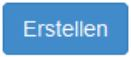
\includegraphics[height=12pt]{Icons/B_Erstellen.jpg} pour créer la séance. 
	\item[$\Longrightarrow$] Vous pouvez ajouter un ordre du jour prédéfini puis appuyer sur 'accepter' et / ou ajouter des points d'ordre du jour un à un avec le bouton 
\includegraphics[height=12pt]{Icons/Pluszeichen.jpg}.
  \item[$\Longrightarrow$] Vous pouvez ajouter des pièces jointes ainsi que des indications de préparation à la séance.					
	\item[$\Longrightarrow$] Cliquez sur 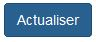
\includegraphics[height=12pt]{Icons/B_Uebernehmen.jpg} pour sauvegarder les informations.
\end{itemize}
\end{tcolorbox}


%% bishierher


\begin{tcolorbox}[colback=blue!5,colframe=blue!40!black,title=Modifier / envoyer une invitation]
\begin{itemize}
  \item[$\Longrightarrow$] Cochez la case 'invitation envoyée' 
\includegraphics[height=12pt]{Icons/sbox_ok.jpg} (en haut à gauche) et la séance apparaîtra dans l'aperçu personnel des personnes invitées.
  \item[$\Longrightarrow$] Vous pouvez soit générer une invitation sous format PDF 
\includegraphics[height=12pt]{Icons/Briefsymbol.jpg} pour ensuite l'envoyer aux invités, soit créer une invitation électronique 
\includegraphics[height=12pt]{Icons/Kalendersymbol.jpg} à envoyer directement aux invités depuis Outlook.
  \item[$\Longrightarrow$] Cliquez sur 
\includegraphics[height=12pt]{Icons/Listensymbol.jpg} pour accéder au procès-verbal de la séance. Vous pouvez rédiger le procès-verbal et ses ordres du jour et définir des affaires en suspens ou des décisions.		
\end{itemize}
\end{tcolorbox}


\end{multicols}

%%%% Box 3+4 in zwei Spalten

\begin{multicols}{2}

\begin{tcolorbox}[colback=blue!5,colframe=blue!40!black,title=Rédiger le procès-verbal]
\begin{itemize}
  \item[$\Longrightarrow$] Dans le procès-verbal de séance (accessible par le symbole 
\includegraphics[height=10pt]{Icons/Listensymbol.jpg}), vous pouvez rédiger le contenu du procès-verbal.
	\item[$\Longrightarrow$] Cliquez sur 
\includegraphics[height=10pt]{Icons/Pfeil_auf-ab.jpg} pour afficher les options :
  \item[$\Longrightarrow$] Les fonctions 
\includegraphics[height=10pt]{Icons/Gutzeichen_Rahmen.jpg} et 
\includegraphics[height=10pt]{Icons/Pfeil_Gutzeichen.jpg} vous permettent d'ajouter une décision ou une affaire en suspens à ce point de l'ordre du jour.
	  \item[$\Longrightarrow$] Les fonctions 
\includegraphics[height=10pt]{Icons/Pfeil_aus_Box.jpg} et 
\includegraphics[height=10pt]{Icons/Pfeil_Pfeil_aus_Box.jpg} vous permettent de convertir le texte sélectionné en décision ou affaire en suspens.
  \item[$\Longrightarrow$] Cliquez sur le bouton 
\includegraphics[height=10pt]{Icons/Blattsymbol.jpg}, pour générer une version PDF du procès-verbal.
	\item[$\Longrightarrow$] Vous pouvez aussi charger un procès-verbal externe. Cliquez sur 'Parcourir' près de 'Charger procès-verbal' et choisissez un fichier.
	\item[$\Longrightarrow$] Une fois le procès-verbal archivé, il n'est plus possible d'y apporter des modifications.
\end{itemize}
\end{tcolorbox}


\begin{tcolorbox}[colback=blue!5,colframe=blue!40!black,title=Listes d'affaires en suspens et de décisions]
\begin{itemize}
  \item[$\Longrightarrow$] Vous pouvez ajouter des décisions ou des affaire en suspens directement depuis un point de l'ordre du jour (en mode de rédaction du procès-verbal).
  \item[$\Longrightarrow$] Vous pouvez également ajouter des décisions et des affaires en suspens en dehors d'un procès-verbal : 
  \item[$\Longrightarrow$] Sélectionnez l'élément du menu 'Gestion de séances' puis le sous-élément 'Affaires en suspens' ou 'Décision'. Vous pouvez alors ajouter une nouvelle affaire en suspens ou décision en cliquant sur le symbole 
\includegraphics[height=9pt]{Icons/Plussymbol.jpg}.
  \item[$\Longrightarrow$] Remplissez les champs désirés en tenant compte des champs obligatoires (*). 
	\item[$\Longrightarrow$] Dans les aperçus des affaires en suspens ou des décisions, vous pouvez rechercher un élément en utilisant la recherche plein texte ou en filtrant les colonnes (ID, titre, type de séance, etc.).
	\item[$\Longrightarrow$] Dans l'aperçu personnel, les affaires en suspens s'affichent avec un cercle de couleur différente selon si le délai est dépassé (
\includegraphics[height=9pt]{Icons/PunktRot.jpg}), s'il approche (
\includegraphics[height=9pt]{Icons/PunktGelb.jpg}) ou s'il est encore loin (
\includegraphics[height=9pt]{Icons/PunktGruen.jpg}).
\end{itemize}
\end{tcolorbox}


\end{multicols}


%%% HINWEISE %%%
%%% Hinweise in 1er Spalte

\begin{beamerlikethm}{Remarques / Astuces}
\begin{itemize}
  \item[$\Longrightarrow$] Au lieu de cliquer 'Parcourir' pour choisir un fichier à charger, vous pouvez glisser et déposer le fichier sur le champ 'Parcourir'.
  \item[$\Longrightarrow$] Vous pouvez changer la structure de l'ordre du jour en utilisant les flèches 
\includegraphics[height=9pt]{Icons/Pfeil-links-rechts.jpg} pour passe du niveau 1 au niveau 1.1 ou pour enlever le numéro.
	\item[$\Longrightarrow$] Le symbole 
\includegraphics[height=9pt]{Icons/UeberarbModus.jpg} permet de travailler en suivi de modifications lors de la modification d'un procès-verbal par un utilisateur.
\end{itemize}
\end{beamerlikethm}

  %%%%%%
	% Spalte 2
	%%%%%%
	
	% Reserve
	
% 	\begin{tcolorbox}[colback=blue!5,colframe=blue!40!black,title=Protokoll bearbeiten]
% \begin{itemize}
%   \item[$\Longrightarrow$] Kehren Sie zur Übersicht zurück
%   \item[$\Longrightarrow$] Wählen Sie die gewünschte Sitzung aus und klicken Sie auf den blauen Titel. Die Optionen öffnen sich
%   \item[$\Longrightarrow$] Klicken Sie auf das Protokollsymbol. Das Sitzungsprotokoll wird geöffnet.
%   \item[$\Longrightarrow$] Sie können das erstellte PDF per Email oder auch per Post versenden.
% \end{itemize}
% \end{tcolorbox}


\pagebreak

\centering{{\huge Beschaffungswesen}}

\vspace{\baselineskip}

%% bishierher

%%%% Box 1+2 in zwei Spalten

\begin{multicols}{2}

\begin{tcolorbox}[colback=blue!5,colframe=blue!40!black,title=(1) Neue Beschaffung initialisieren]
\begin{itemize}
  \item[$\Longrightarrow$] Vorbereitung: Erstellen Sie sämtliche Dokumente zur Offertenanfrage ausserhalb von CUBE PA.
  \item[$\Longrightarrow$] Klick auf 
\includegraphics[height=10pt]{Icons/Plussymbol.jpg} und füllen Sie alle benötigten Felder aus.
  \item[$\Longrightarrow$] Beachten Sie die Pflichtfelder. Der Status ist 'Erstellung Ausschreibung'
  \item[$\Longrightarrow$] Klicken Sie auf 'Übernehmen' oben in der Mitte des Bildes oder auf 'Erstellen' unterhalb der Felder.
	\item[$\Longrightarrow$] Erst jetzt ist es Möglich die Ausschreibungsunterlagen hochzuladen.
  \item[$\Longrightarrow$] Schliessen Sie diesen Vorgang ebenfalls mit 'Übernehmen' ab. Die Ausschreibung wurde erstellt.
	\item[$\Longrightarrow$] Dokumentenprüfung und Fertigstellung durch Kunde.
\end{itemize}
\end{tcolorbox}


%% bishierher


\begin{tcolorbox}[colback=blue!5,colframe=blue!40!black,title=(2) Offertanfrage versenden]
\begin{itemize}
  \item[$\Longrightarrow$] Gewünschte Beschaffung öffnen. Falls die gewünschten 'Eingeladenen' nicht auf der Liste sind, mit Administrator Kontakt aufnehmen.
	\item[$\Longrightarrow$] Klick auf 'Senden' 
\includegraphics[height=12pt]{Icons/Versandsymbol.jpg}. Auswahl Versand per Email oder Brief.
  \item[$\Longrightarrow$] Email: Emailvorlage mit Link wird erstellt. Brief: Briefvorlage mit Einladungstext wird erstellt (pdf).
  \item[$\Longrightarrow$] Status ändern auf 'Ausschreibung versendet'. Vorgang abschliessen mit 'Übernehmen'.
\end{itemize}
\end{tcolorbox}


\end{multicols}

%%%% Box 3+4 in zwei Spalten

\begin{multicols}{2}

\begin{tcolorbox}[colback=blue!5,colframe=blue!40!black,title=(3) Offerte(n) entgegennehmen und prüfen]
\begin{itemize}
  \item[$\Longrightarrow$] Eingehende Offerten in CUBE erfassen (Beschaffungswesen/Offerten) und mit Beschaffung verknüpfen:
	\item[$\Longrightarrow$] Für die eingegangene Offerte zugehörige Beschaffung auswählen.
  \item[$\Longrightarrow$] Alle nötigen Felder ausfüllen und Pflichtfelder beachten. Mit 'Erstellen' werden Angaben gespeichert.
	\item[$\Longrightarrow$] Erst nach 'Erstellen' können Dokumente hochgeladen werden: Offerte hochladen. Abschliessen mit 'Übernehmen'.
	\item[$\Longrightarrow$] Status in der entsprechenden Beschaffung auf 'Offertprüfung' ändern.
\end{itemize}
\end{tcolorbox}


\begin{tcolorbox}[colback=blue!5,colframe=blue!40!black,title=(4) Vergabeantrag ausfüllen]
\begin{itemize}
  \item[$\Longrightarrow$] Datum des Vergabeantrages eingeben und gewünschte Beschaffung auswählen.
  \item[$\Longrightarrow$] Zum Zuschlag empfohlene Offerte auswählen, Kommentar einfügen und mit 'Erstellen' speichern.
  \item[$\Longrightarrow$] Beilagen können erst nach 'Erstellen' hinzugefügt werden. Abschliessen mit 'Übernehmen'.
	\item[$\Longrightarrow$] Status in der entsprechenden Beschaffung auf 'Vergabeantrag an Kunde' ändern. Nach Genehmigung auf 'Vergabe erfolgt'.
	\item[$\Longrightarrow$] \textbf{Hinweis:} Der Vergabeantrag dient als Sicherung gegen Nachträgliche Änderungen.
\end{itemize}
\end{tcolorbox}


\end{multicols}

%%% 5te Kachel, 1-spaltig, blau

% \begin{multicols}{1}
\begin{tcolorbox}[colback=blue!5,colframe=blue!40!black,title=(5) Vertrag ausstellen / Abschluss der Beschaffung]
\begin{itemize}
  \item[$\Longrightarrow$] Vertragsdokument / Auftrag erstellen. In 'Beschaffung/Verträge' Vertrag erfassen und mit Offerte verknüpfen.
	\item[$\Longrightarrow$] In CUBE wird vorerst das nicht unterschriebene Schreiben hochgeladen (erst möglich nach 'Erstellen').
  \item[$\Longrightarrow$] Info an Kunde über bereitliegende Vertragsdokumente: Kontrolle, Unterschrift Auftraggeber und Auftragnehmer.
	\item[$\Longrightarrow$] Unterschriebene Dokumente in CUBE hochladen. Status in der entsprechenden Beschaffung auf 'Vertrag abgeschlossen' ändern.
	\item[$\Longrightarrow$] Absageschreiben erstellen und versenden.
	\item[$\Longrightarrow$] \textbf{Hinweis:} Ist gewünschte Firma nicht unter 'Auftragnehmer' aufgelistet, bitte mit dem Administrator Kontakt aufnehmen.
\end{itemize}
\end{tcolorbox}
% \end{multicols}


%%% HINWEISE %%%
%%% Hinweise in 1er Spalte, roter Rahmen

% \begin{beamerlikethm}{(5) Vertrag ausstellen / Abschluss der Beschaffung}
% \begin{itemize}
%  \item[$\Longrightarrow$] Vertragsdokument / Auftrag erstellen. In 'Beschaffung/Verträge' Vertrag erfassen und mit Offerte verknüpfen.
%	\item[$\Longrightarrow$] In CUBE wird vorerst das nicht unterschriebene Schreiben hochgeladen (erst möglich nach 'Erstellen').
%  \item[$\Longrightarrow$] Info an Kunde über bereitliegende Vertragsdokumente: Kontrolle, Unterschrift Auftraggeber und Auftragnehmer.
%	\item[$\Longrightarrow$] Unterschriebene Dokumente in CUBE hochladen. Status in der entsprechenden Beschaffung auf 'Vertrag abgeschlossen' ändern.
%	\item[$\Longrightarrow$] Absageschreiben erstellen und versenden.
% \end{itemize}
% \end{beamerlikethm}

  %%%%%%
	% Spalte 2
	%%%%%%
	
	% Reserve
	
% 	\begin{tcolorbox}[colback=blue!5,colframe=blue!40!black,title=Protokoll bearbeiten]
% \begin{itemize}
%   \item[$\Longrightarrow$] Kehren Sie zur Übersicht zurück
%   \item[$\Longrightarrow$] Wählen Sie die gewünschte Sitzung aus und klicken Sie auf den blauen Titel. Die Optionen öffnen sich
%   \item[$\Longrightarrow$] Klicken Sie auf das Protokollsymbol. Das Sitzungsprotokoll wird geöffnet.
%   \item[$\Longrightarrow$] Sie können das erstellte PDF per Email oder auch per Post versenden.
% \end{itemize}
% \end{tcolorbox}



\end{document}